
\documentclass[
	%twocolumn, % Use two-column layout for the document.
	secnumarabic, % Number sections and subsections with Arabic numerals (e.g., IV.1 instead of letters).
	nobibnotes, % Suppress the use of footnotes in bibliography entries.
	aps, % Specify the American Physical Society document style.
	prb, % Use the style for Physical Review B (often for condensed matter and materials physics).
	floatfix, % Attempt to resolve issues with floats (e.g., figures or tables) being placed improperly.
	% superscriptaddress, % Format author affiliations as superscripts rather than inline.
]{revtex4-2}

\usepackage[utf8]{inputenc} % Input Encoding
\usepackage[T1]{fontenc} % Font Encoding
\usepackage{lmodern} % Show umlauts as vector graphics

\usepackage{
	amsmath, mathtools, % math
	bm, % bold math
	amssymb, % fonts from American Pysical Society, e.g., \mathbb
	subcaption,
	xcolor, % colors like \color{red}
}

\usepackage{hyperref}
\hypersetup{
	colorlinks=true,
	linkcolor=blue,
	filecolor=magenta,
	urlcolor=cyan,
}
% cleveref: better "ref" commands with "cref".
% load cleveref after other referencing packages, e.g., hyperref
% see also: https://tex.stackexchange.com/questions/36295/cross-reference-packages-which-to-use-which-conflict
\usepackage[capitalize]{cleveref}
\crefname{section}{Sec.}{Secs.}
\crefname{subsection}{Subsec.}{Subsecs.}


% see also https://www.namsu.de/Extra/pakete/Caption.html for an overview
% \captionsetup{
% 	justification=justified,
% 	format=plain,
% 	singlelinecheck=true,
% 	margin=10pt
% }

% \captionsetup[subfigure]{
% 	justification=raggedright,
% 	singlelinecheck=false,
% 	margin=0pt,
% 	skip=0pt,
% }

\newcommand{\todo}[1]{{\color{red}TODO: #1}}


\begin{document}

\title{Quantum Hall effect}

\author{Valerii Kozin}
\author{Maximilian Hünenberger}

\maketitle


\begin{figure}[htbp]
	\centering
	% First row
	\begin{subcaptiongroup}
		\begin{subfigure}{0.3\textwidth}
			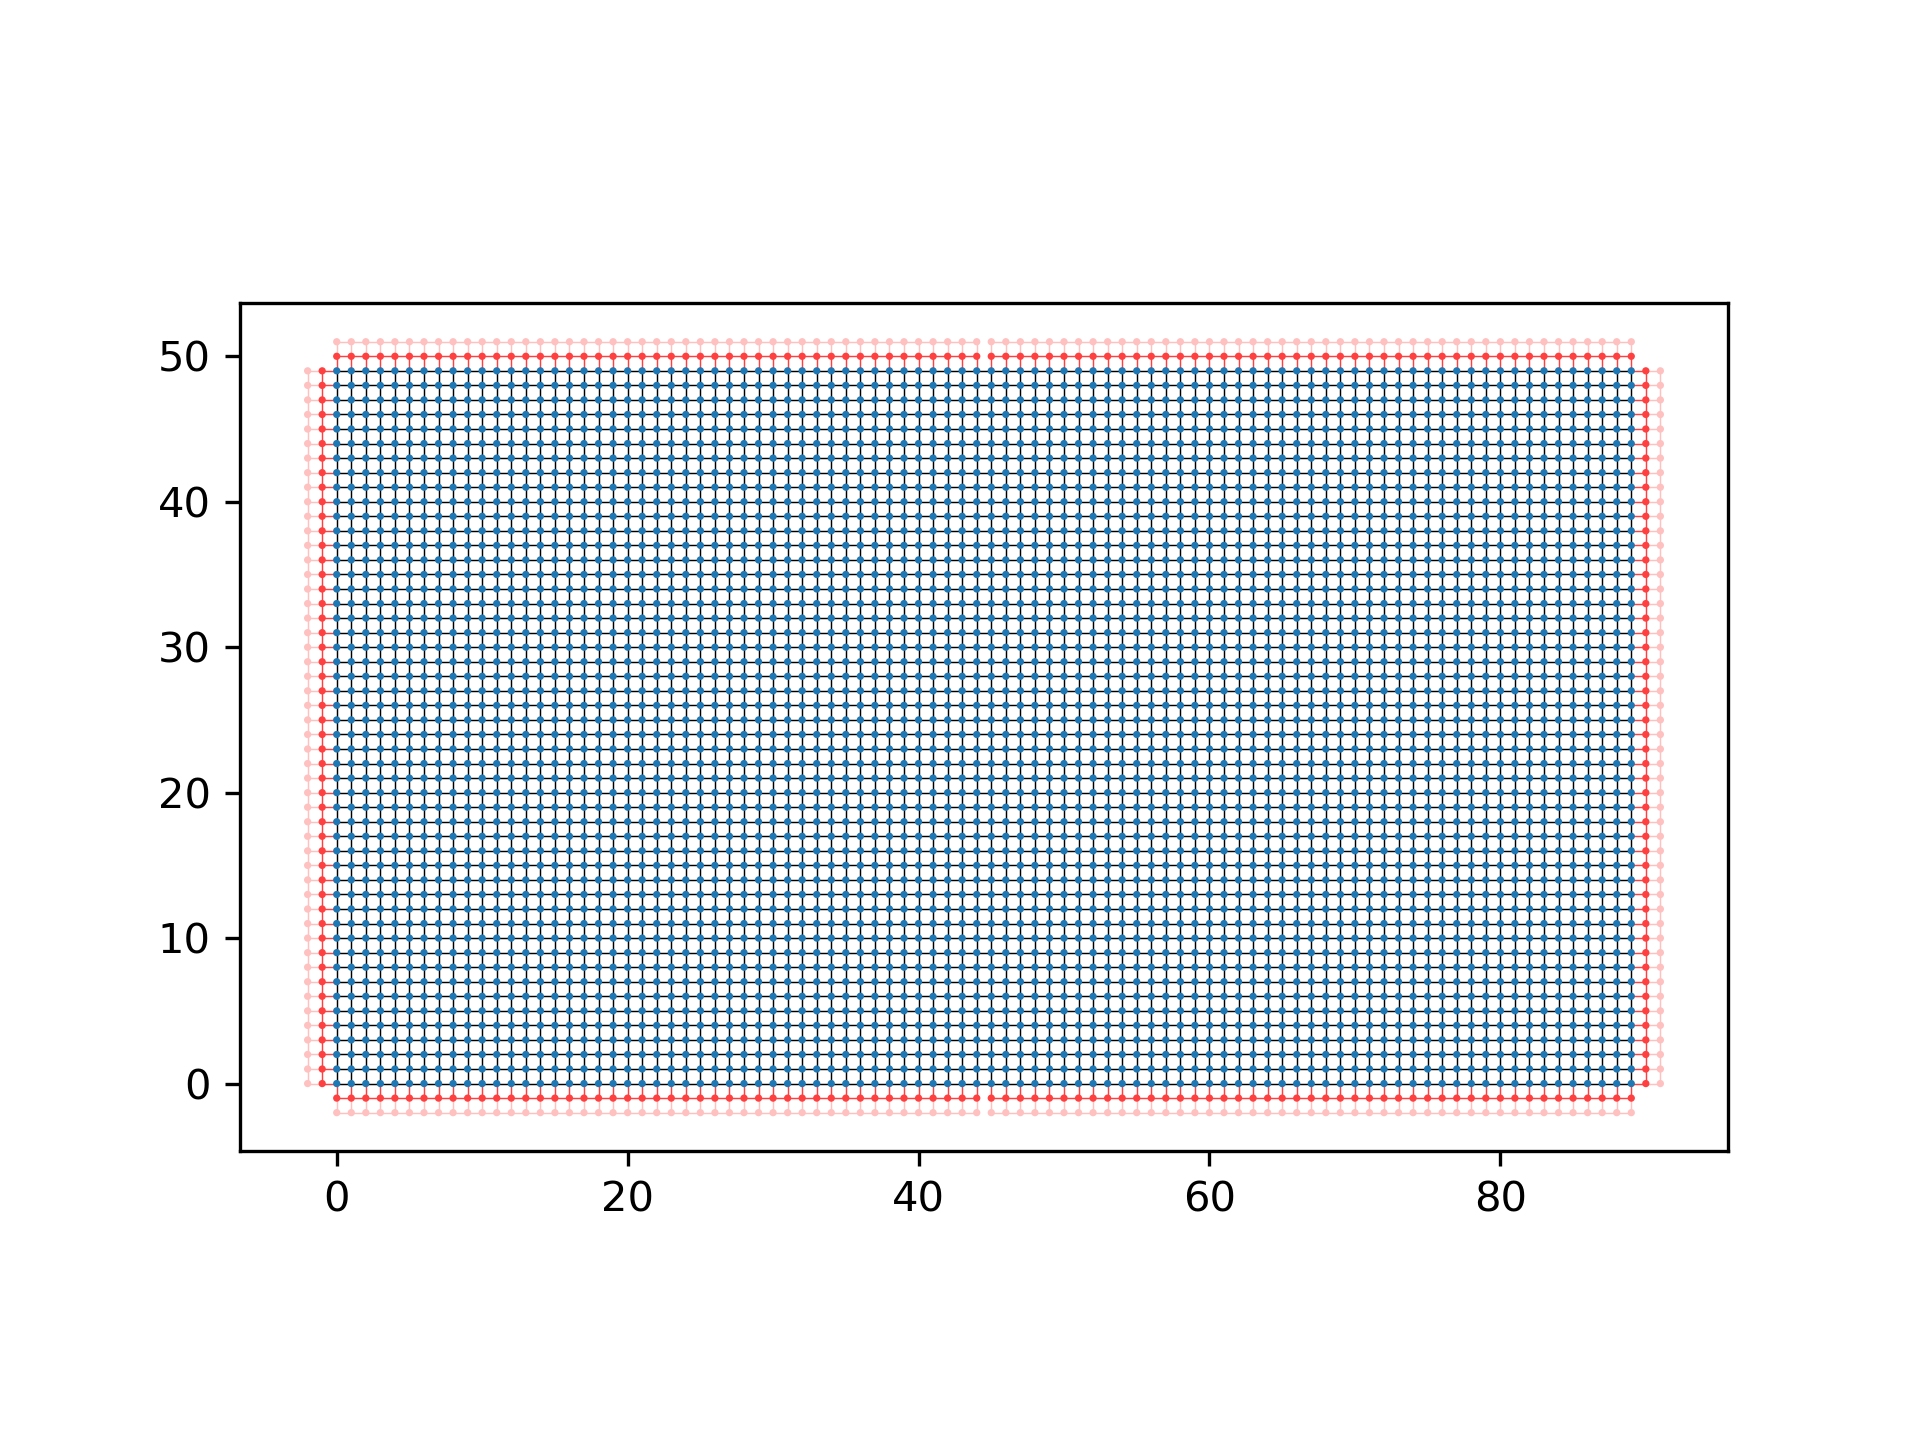
\includegraphics[width=\linewidth]{Figures/lead width and B field/system wide leads.png}
			\caption{System with wide leads}
		\end{subfigure}
		\hfill
		\begin{subfigure}{0.3\textwidth}
			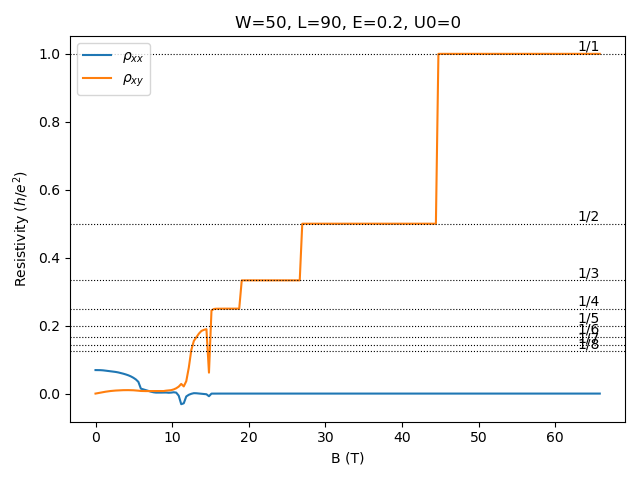
\includegraphics[width=\linewidth]{Figures/lead width and B field/B in wide leads hall_W50_L90_E0.2_U00_T0_phi0-0.1_nphis201_nseeds1_temp0_BinLeadsTrue.png}
			\caption{$B$-field in wide leads}
			\label{fig: Resistivity(B): B field in wide leads}
		\end{subfigure}
		\hfill
		\begin{subfigure}{0.3\textwidth}
			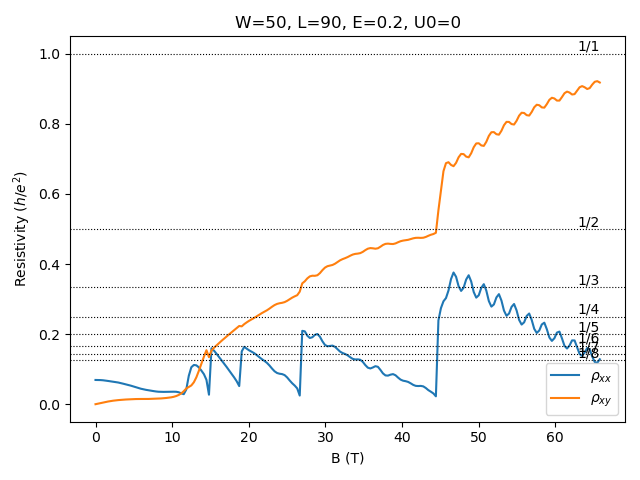
\includegraphics[width=\linewidth]{Figures/lead width and B field/no B in wide leads hall_W50_L90_E0.2_U00_T0_phi0-0.1_nphis201_nseeds1_temp0_BinLeadsFalse.png}
			\caption{No $B$-field in wide leads}
		\label{fig: Resistivity(B): No B field in wide leads}
		\end{subfigure}
	\end{subcaptiongroup}

	\vspace{1em}

	% Second row
	\begin{subcaptiongroup}
		\begin{subfigure}{0.3\textwidth}
			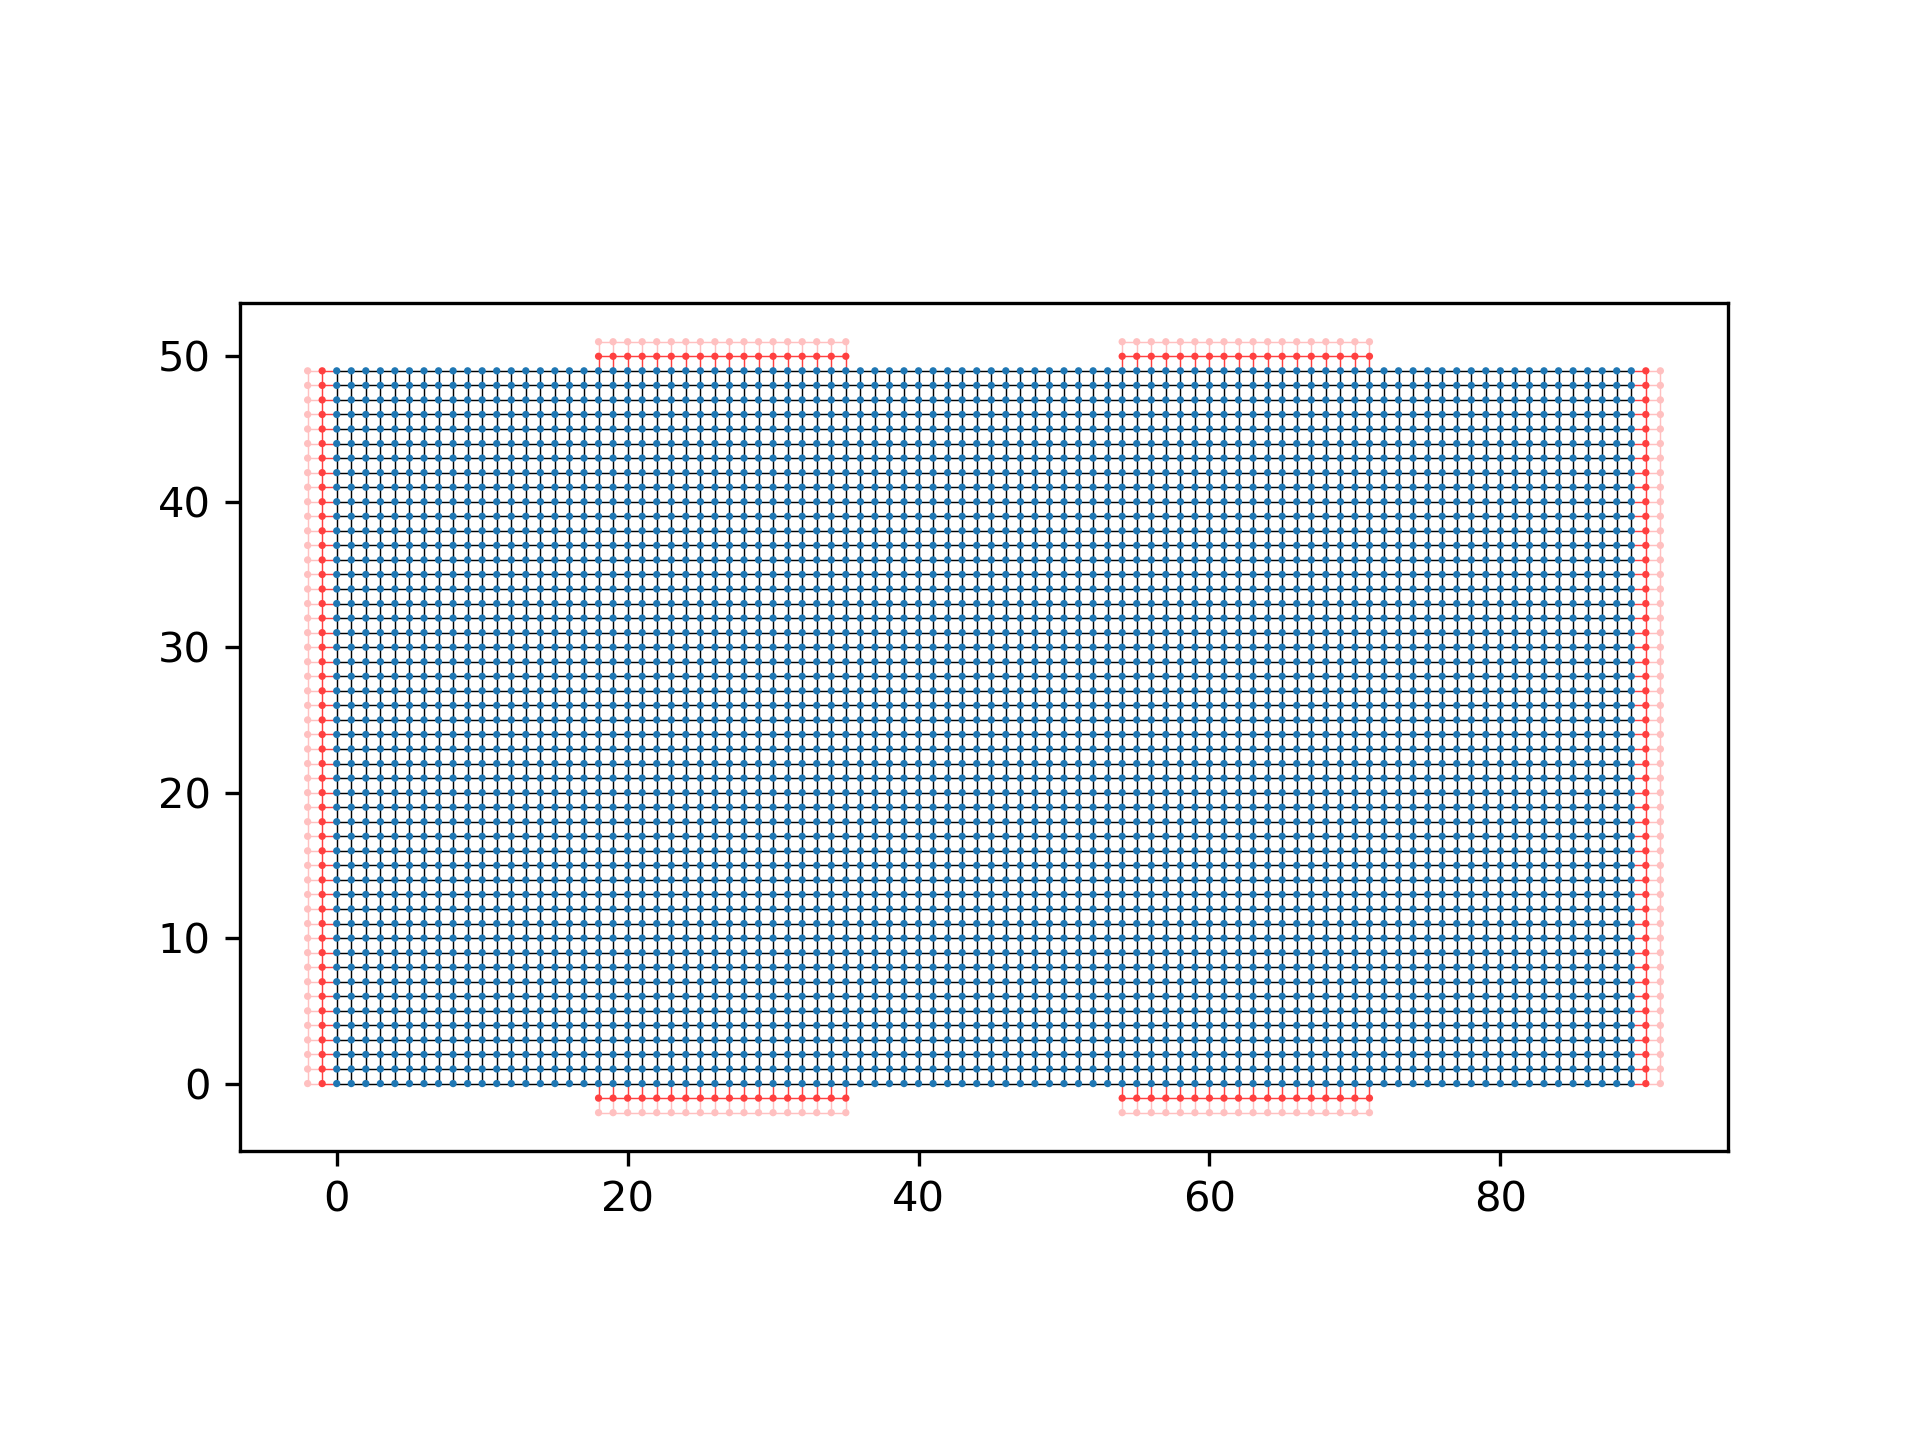
\includegraphics[width=\linewidth]{Figures/lead width and B field/system narrow leads.png}
			\caption{System with narrow leads ($L/5$)}
		\end{subfigure}
		\hfill
		\begin{subfigure}{0.3\textwidth}
			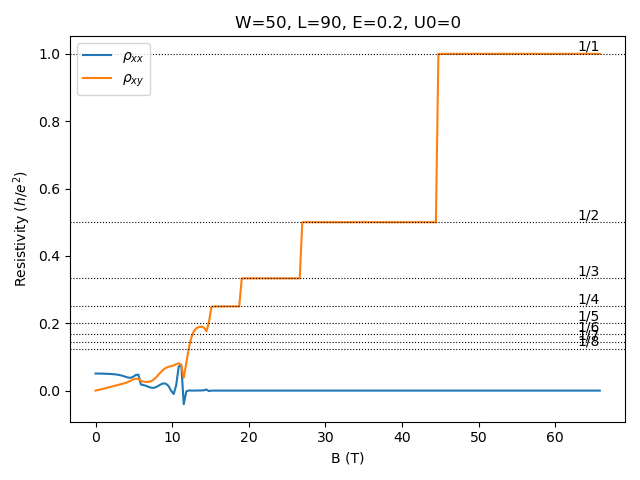
\includegraphics[width=\linewidth]{Figures/lead width and B field/B in narrow Ldiv5 leads hall_W50_L90_E0.2_U00_T0_phi0-0.1_nphis201_nseeds1_temp0_BinLeadsTrue.png}
			\caption{$B$-field in narrow leads}
			\label{fig: Resistivity(B): B field in narrow leads}
		\end{subfigure}
		\hfill
		\begin{subfigure}{0.3\textwidth}
			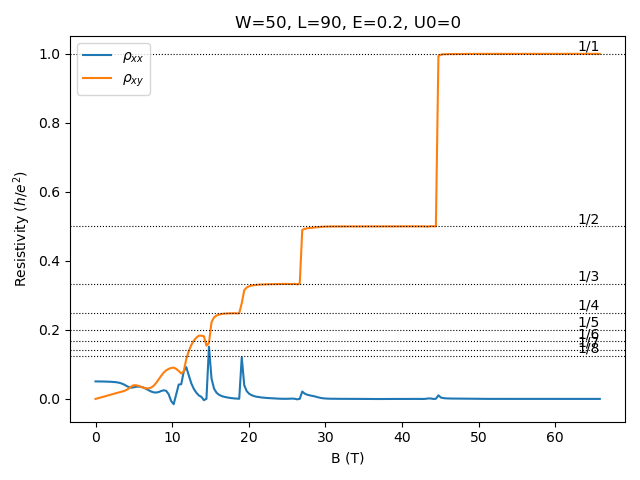
\includegraphics[width=\linewidth]{Figures/lead width and B field/no B in narrow Ldiv5 leads hall_W50_L90_E0.2_U00_T0_phi0-0.1_nphis201_nseeds1_temp0_BinLeadsFalse.png}
			\caption{No $B$-field in narrow leads}
			\label{fig: Resistivity(B): No B field in narrow leads}
		\end{subfigure}
	\end{subcaptiongroup}

	\caption{Comparison of resistivities as a function of magnetic field for wide/narrow leads with and without $B$-field inside them (i.e., Peierls phase).}
	\label{fig: Resistivity(B) wide narrow leads with and without B}
\end{figure}

In
	\cref{fig: Resistivity(B) wide narrow leads with and without B}
	we observe that except for
	\cref{fig: Resistivity(B): No B field in wide leads}
	all Hall-resistivities $\rho_{xy}$ have similar plateaus.
This is likely due to the fact that the edge state is not preserved in leads without $B$-field.
Thus, for wide leads there is more scattering which smears out the plateaus and increases the longitudinal resistivity $\rho_{xx}$.
If there is no $B$-field in narrow leads
	[see \cref{fig: Resistivity(B): No B field in narrow leads}]
	the $\rho_{xx}$ is pronounced when the bulk is conducting, since \todo{explain}


\end{document}